\chapter{基础知识}
\begin{mathchapterlayout}

本章建立理解后续设计所需的理论基础。内容从格与模运算开始，依次说明格困难问题、环对象的
系数与频域表示、离散Gaussian、格陷门及低秩线性代数，再介绍HIBE、IBS和IB-ME的基本语法。
这些概念构成描述身份基密码与结构化格运算的数学工具。

\section{数学符号与格基础}

\subsection{向量、矩阵与模运算}

记整数集合为$\mathbb Z$，模$q$整数环为$\mathbb Z_q=\mathbb Z/q\mathbb Z$。其中每个元素
表示一个同余类，满足$x\equiv y\pmod q$当且仅当$q$整除$x-y$。同一同余类在$[0,q)$中
具有唯一的非负整数代表元，在$(-q/2,q/2]$中具有唯一的中心整数代表元。模运算在同余类上
进行；范数描述所选整数向量的大小。

对向量$\mathbf x=(x_1,\ldots,x_n)$，报告主要使用欧氏范数和无穷范数
\[
 \lVert\mathbf x\rVert_2=\sqrt{\sum_{i=1}^{n}x_i^2},
 \qquad
 \lVert\mathbf x\rVert_\infty=\max_i|x_i|.
\]
签名方案通常要求响应向量满足给定范数界；加密方案则要求误差足够小，使解密时能够区分编码
区间。各方案以公开参数$pp$记录维数、模数、范数界及采样配置。

表~\ref{tab:foundation-symbols}列出后文频繁使用的符号。

\begin{table}[H]
\centering\small
\caption{基础数学符号}
\label{tab:foundation-symbols}
\begin{tabularx}{\textwidth}{@{}p{.22\textwidth}X@{}}
\toprule
\rowcolor{black!8} 符号 & 含义 \\
\midrule
$n,m,d,k,\ell$ & 格维数、矩阵宽度、环次数或模块秩等整数参数，具体含义由方案给出 \\
$q$ & 模数；$\mathbb Z_q$表示模$q$整数环 \\
$A,\mathbf a$ & 公开矩阵或公开向量 \\
$\mathbf s,\mathbf e$ & 秘密向量与小误差向量 \\
$\lVert\cdot\rVert_2,\lVert\cdot\rVert_\infty$ & 欧氏范数与无穷范数 \\
$R_q$ & 多项式商环$\mathbb Z_q[x]/(f(x))$ \\
$D_{\Lambda,s,\mathbf c}$ & 格$\Lambda$上中心为$\mathbf c$、宽度为$s$的离散Gaussian分布 \\
\bottomrule
\end{tabularx}
\end{table}

\subsection{格、$q$元核格与目标陪集}

给定线性无关向量组成的基$B=[\mathbf b_1,\ldots,\mathbf b_n]\in\mathbb R^{m\times n}$，
由$B$生成的格为
\[
  \Lambda(B)=\{B\mathbf z:\mathbf z\in\mathbb Z^n\}.
\]
同一个格可以具有许多不同的基，基的几何质量会影响求近向量和Gaussian采样等算法。早期格陷门通常采用一组短而较好正交的格向量；后来的结构化陷门采用短矩阵等秘密辅助信息。公开对象通常表示为模矩阵或环向量
\cite{gpv2008,micciancio2012trapdoors}。

模$q$矩阵$A\in\mathbb Z_q^{n\times m}$定义从$\mathbb Z^m$到$\mathbb Z_q^n$的映射
$\mathbf x\mapsto A\mathbf x\bmod q$。该映射的核为$q$元核格
\[
 \Lambda_q^\perp(A)=\{\mathbf x\in\mathbb Z^m:A\mathbf x=\mathbf0\pmod q\},
\]
给定目标$\mathbf u$时，相应解集为
\[
 \Lambda_q^{\mathbf u}(A)=\{\mathbf x\in\mathbb Z^m:A\mathbf x=\mathbf u\pmod q\}.
\]
若$\mathbf x_0$是其中一个解，则
\[
 \Lambda_q^{\mathbf u}(A)=\mathbf x_0+\Lambda_q^\perp(A).
\]
因此，$\Lambda_q^{\mathbf u}(A)$是核格的一个目标陪集，由核格平移$\mathbf x_0$得到。身份基发钥和格签名经常需要在该陪集中找到满足分布与范数要求
的短向量。陷门帮助合法持有者高效完成满足目标方程的短原像采样。

\section{格上困难问题及结构变体}

\subsection{LWE问题}

学习带误差问题（Learning With Errors，LWE）由Regev系统提出并用于构造公钥密码
\cite{regev2005lwe}。取均匀矩阵$A\in\mathbb Z_q^{m\times n}$、秘密$\mathbf s\in\mathbb
Z_q^n$和小误差$\mathbf e\in\mathbb Z^m$，观察值为
\[
  \mathbf b=A\mathbf s+\mathbf e\pmod q.
\]
搜索型LWE要求从$(A,\mathbf b)$恢复$\mathbf s$；判定型LWE要求区分$(A,\mathbf b)$与均匀
样本。若没有误差，线性方程可以直接求解；小误差使恢复秘密成为格上的困难问题。格加密通常将
明文或封装种子叠加在这类带误差关系上，合法密钥可以消去主线性项并解码小扰动。

\subsection{SIS问题}

短整数解问题（Short Integer Solution，SIS）与Ajtai建立的平均情形格问题有关
\cite{ajtai1996}。给定均匀矩阵$A\in\mathbb Z_q^{n\times m}$，目标是找到非零短向量
$\mathbf z$，满足
\[
 A\mathbf z=\mathbf0\pmod q,
 \qquad 0<\lVert\mathbf z\rVert_2\leq\beta.
\]
非齐次版本给出目标$\mathbf u$，要求寻找短向量$\mathbf z$使$A\mathbf z=\mathbf u\pmod q$。
格签名常把身份和消息哈希为目标向量，再由陷门采样满足方程的短原像。验证者检查模方程和范数，
而不知道陷门的参与者难以为新目标构造合格短向量。

\subsection{环格、模格与NTRU结构}

普通矩阵格以$\mathbb Z_q$上的矩阵和向量描述代数关系。环格利用多项式商环上的结构，常取
\[
 R_q=\mathbb Z_q[x]/(x^N+1)
\]
作为基础环，其中$N$通常为2的幂。每个环元素都可唯一写成
$a_0+a_1x+\cdots+a_{N-1}x^{N-1}$，因而只需保存$N$个模$q$系数。由于商环中$x^N=-1$，
乘积超过$N-1$次的项折回时改变符号；若$c(x)=a(x)b(x)$，则
\[
 c_k=\sum_{i+j=k}a_i b_j-\sum_{i+j=k+N}a_i b_j\pmod q,
 \qquad 0\leq k<N.
\]
这就是负循环乘法。一个$r\times t$环矩阵包含$Nrt$个系数，其作用等价于一个更大的结构化
系数矩阵。多项式表示将这一结构保存在系数关系中，Ring-LWE和Ring-SIS由此获得紧凑表示和
快速多项式运算\cite{lpr2013ring}。

模格在$R_q$上使用低秩向量或矩阵，在普通矩阵格的灵活性和环格的结构性之间折中；对应问题通常
称为Module-LWE与Module-SIS\cite{langlois2015module}。模块秩为1时对应环上的关系；增大
模块秩可以在多项式次数之外进一步调整代数维度。

NTRU结构同样在多项式环上运算，通过短多项式关系形成结构化格。该结构可以用于加密、签名和
陷门委派。不同格结构以矩阵、环向量或短多项式关系描述公开映射与秘密信息，并对应不同的
困难问题假设。

\subsection{环伴随与频域表示}

对实系数环元素$f(x)=\sum_{i=0}^{N-1}f_i x^i$，定义环上的伴随
\[
 f^\star(x)=f(x^{-1})\bmod(x^N+1)
 =f_0-\sum_{i=1}^{N-1}f_i x^{N-i}.
\]
对环矩阵，$T^\star$表示先转置再对每个元素取上述伴随。取
$\omega_j=\exp((2j+1)\pi\mathrm i/N)$，在$x^N+1$的复根上计算$f(\omega_j)$，即可得到负循环
Fourier表示。此时环乘法在每个频率上变为复数乘法，并且
$f^\star(\omega_j)=\overline{f(\omega_j)}$；环矩阵的伴随相应变为复矩阵的共轭转置。实系数对象的
频率值成共轭对，一半频率的取值即可通过共轭对称性确定其余取值。

系数表示给出多项式的整数系数，Fourier表示给出同一多项式在各复根上的取值。两种表示由
正、逆变换联系，负循环卷积在频域化为逐点乘法；整数系数上的同余关系则由模$q$运算描述。

\begin{table}[H]
\centering\small
\caption{常见格结构及其代数表示}
\label{tab:lattice-families}
\begin{tabularx}{\textwidth}{@{}p{.18\textwidth}p{.25\textwidth}X@{}}
\toprule
\rowcolor{black!8} 结构 & 典型对象 & 结构特征 \\
\midrule
普通矩阵格 & $\mathbb Z_q$上的矩阵与整数向量 & 表达直接，目标参数下矩阵和陷门对象可能较大 \\
环格 & 商环多项式与环向量 & 可利用卷积和频域结构，需处理环采样与数值变换 \\
模格 & 小秩环向量或环矩阵 & 在结构复用与方案灵活性之间折中 \\
NTRU结构格 & 满足短多项式关系的结构化基 & 对象较紧凑，可支持快速签名、加密和陷门委派 \\
\bottomrule
\end{tabularx}
\end{table}

\section{离散Gaussian与格陷门}

\subsection{离散Gaussian采样}

对格$\Lambda$、中心$\mathbf c$和宽度$s>0$，连续Gaussian权重写为
\[
 \rho_{s,\mathbf c}(\mathbf x)=
 \exp\!\left(-\pi\frac{\lVert\mathbf x-\mathbf c\rVert_2^2}{s^2}\right).
\]
令$\rho_{s,\mathbf c}(\Lambda)=\sum_{\mathbf y\in\Lambda}\rho_{s,\mathbf c}(\mathbf y)$，离散
Gaussian分布的完整概率为
\[
 \Pr[X=\mathbf x]
 =\frac{\rho_{s,\mathbf c}(\mathbf x)}{\rho_{s,\mathbf c}(\Lambda)},
 \qquad \mathbf x\in\Lambda.
\]
GPV与MP12采用上述以$\pi$归一化的Gaussian权重，宽度参数为$s$。相应一维连续Gaussian的
标准差为$\sigma=s/\sqrt{2\pi}$，其权重也可写为$\exp(-\lVert\mathbf x-\mathbf c\rVert^2/(2\sigma^2))$；因此$s=\sqrt{2\pi}\sigma$\cite{gpv2008,micciancio2012trapdoors}。

当分布定义在$q$元核格的目标陪集上时，样本同时满足给定模方程。宽度$s$决定概率质量围绕
中心的集中程度，并影响向量范数和分布的统计性质。格密码中的采样参数由平滑条件、陷门质量
与目标向量长度共同确定。

格上的Gaussian采样可以借助格基的Gram--Schmidt正交信息，或利用结构化陷门把高维目标
分解为较低维的陪集问题。扰动采样先产生具有相关性的随机向量，再结合目标陪集上的离散
采样，形成所需的分布。

\subsection{陷门生成、委派与短原像采样}

格陷门是一份能够帮助合法持有者完成短原像采样的秘密辅助信息。典型算法可以概括为：

\begin{enumerate}
  \item $\mathsf{TrapGen}$生成统计上接近均匀的公开矩阵$A$及短陷门$T_A$；
  \item $\mathsf{SamplePre}(A,T_A,\mathbf u)$为目标$\mathbf u$采样短向量$\mathbf x$，使
        $A\mathbf x=\mathbf u\pmod q$；
  \item 委派算法把已有陷门扩展到包含新身份块的公开矩阵，同时保持可用的短基或结构化陷门。
\end{enumerate}

GPV采样器以短格基或短满秩向量集为
秘密几何信息；Micciancio--Peikert（MP12）直接使用一份小范数矩阵作为结构化陷门\cite{gpv2008,micciancio2012trapdoors}。Lai等人又将MP12型陷门扩展到
理想格，以环元素代替相应的结构化矩阵块\cite{lai2015trapdoors}。

\subsection{gadget矩阵与结构化陷门}

MP12框架从一个容易求逆和采样的公开gadget矩阵出发。令$k=\lceil\log_2q\rceil$、
$\mathbf g^T=(1,2,\ldots,2^{k-1})$，则常见二进制gadget为
\[
 G=I_n\otimes\mathbf g^T\in\mathbb Z_q^{n\times nk}.
\]
$G$将$n$个二进制分解映射组成分块对角矩阵。每个坐标都可按权重$1,2,\ldots,2^{k-1}$
分解，因而求目标$\mathbf u$的原像可分别处理其$n$个坐标。

对于公开矩阵$A$，MP12型$G$-陷门是一份短矩阵$R$，使
\[
 A\begin{bmatrix}R\\I\end{bmatrix}=HG\pmod q,
\]
其中$H$是可逆标签。生成时可取
\[
 A=[\bar A\mid HG-\bar A R].
\]
合法持有者先把一般目标转换为gadget上的低维预像问题，再结合扰动采样得到$A\mathbf x=\mathbf u
\pmod q$的短解。HIBE的委派进一步为扩展后的身份矩阵生成新陷门；原生格IBS则用短原像作为
身份密钥或签名。图~\ref{fig:preimage-sampling-foundation}归纳各对象的关系。

\begin{figure}[!htbp]
\centering
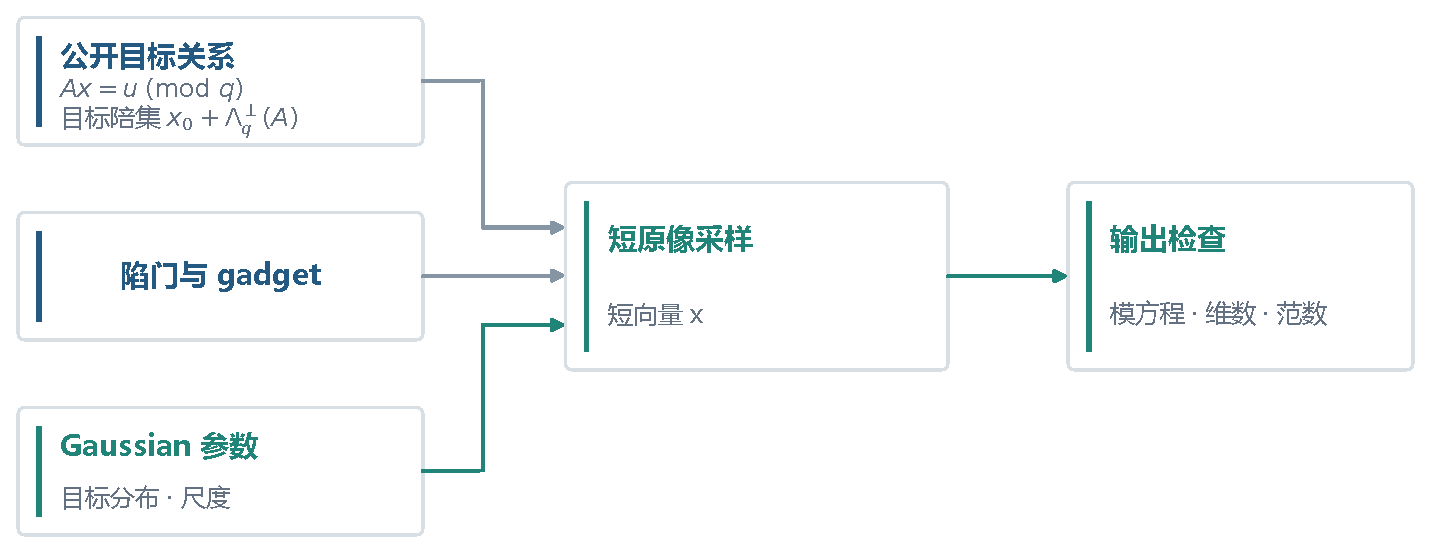
\includegraphics[width=\linewidth,height=.62\textheight,keepaspectratio]{figures/fig-02-01-preimage.pdf}
\caption{目标陪集、陷门、Gaussian参数与短原像之间的关系}
\label{fig:preimage-sampling-foundation}
\end{figure}

公开映射确定目标陪集，秘密陷门提供短原像采样所需的几何信息，Gaussian参数规定样本的
分布与长度。这三者共同构成陷门采样的基本关系。

\section{频域表示与低秩线性代数}

\subsection{Gram矩阵与低维子空间}

对复矩阵$J\in\mathbb C^{r\times k}$，$J^*$表示共轭转置，
\[
 G_J=J^*J\in\mathbb C^{k\times k}
\]
称为$J$的Gram矩阵。对任意$\mathbf y$都有
$\mathbf y^*G_J\mathbf y=\lVert J\mathbf y\rVert_2^2\geq0$，所以$G_J$为半正定矩阵。它记录
$J$各列之间的内积关系；$J^*J$与$JJ^*$的非零特征值相同。当$k\ll r$时，分析
$k\times k$的$J^*J$通常比展开$r\times r$的$JJ^*$更经济。

若$J^*J=U\operatorname{diag}(\lambda_i)U^*$，特征向量给出$J$列空间中的正交方向，特征值描述
这些方向的伸缩程度。与$\operatorname{span}(J)$正交的向量$\mathbf x$满足$J^*\mathbf x=0$，
因此任何形如$JJ^*$的修正项都不会作用在该正交补上。这是后文把大空间运算转入低维子空间的
基本依据。

\subsection{Gaussian参数矩阵与平方根作用}

对正定矩阵$\Sigma$，非球形Gaussian可以写成
\[
 \rho_{\sqrt\Sigma}(\mathbf x)
 =\exp(-\pi\mathbf x^*\Sigma^{-1}\mathbf x).
\]
其中$\Sigma$为Gaussian平方参数矩阵；在上述$\pi$归一化下，连续概率分布的协方差为$\Sigma/(2\pi)$。

若$L L^*=\Sigma$，把标准连续Gaussian向量经过$L$变换即可得到由$\Sigma$描述的相关方向。
当
\[
 \Sigma=aI-cJJ^*,\qquad a,c>0,
\]
修正只发生在$J$的列空间；其正交补仍按$\sqrt a$缩放，而列空间内各方向根据
$a-c\lambda_i$调整。因而可以通过较小的Gram矩阵$J^*J$构造平方根作用，而无须保存完整
$r\times r$矩阵。将这一关系用于环矩阵时，Fourier变换把环乘法分解到各频率，每个频率
对应一个低维复矩阵问题，低秩结构可分别作用于这些矩阵。

\section{身份基加密与分层身份基加密}

\subsection{身份基加密}

身份基加密（Identity-Based Encryption，IBE）使用身份字符串代替传统用户公钥。可信发钥
机构运行$\mathsf{Setup}$得到主公钥$\mathsf{mpk}$和主私钥$\mathsf{msk}$；用户通过
$\mathsf{Extract}(\mathsf{msk},\mathsf{id})$领取身份私钥；发送者以$\mathsf{id}$和
$\mathsf{mpk}$加密；接收者使用对应身份私钥解密。其正确性要求对任意合法身份和消息，诚实
生成的身份私钥能够恢复消息。

IBE把公钥发现问题转换为身份规范与发钥机构管理问题。通信者使用对方规范身份和系统主公钥进行加密，发钥机构负责核验身份、保护主私钥并管理密钥生命周期。因而，IBE适合具有明确组织
边界和统一身份管理的系统。

\subsection{HIBE的分层身份与密钥委派}

分层身份基加密（Hierarchical Identity-Based Encryption，HIBE）把身份扩展为路径
$(\mathsf{id}_1,\ldots,\mathsf{id}_d)$。除$\mathsf{Setup}$、$\mathsf{Extract}$、
$\mathsf{Encrypt}$和$\mathsf{Decrypt}$外，HIBE还包含密钥委派$\mathsf{Derive}$：持有前缀
路径密钥的实体可以为下一层身份生成子密钥，无需再次调用根主私钥。

在两层身份匹配构造中，可将第一层设为接收身份$r$、第二层设为发送身份$s$：
\[
  (\mathsf{id}_1,\mathsf{id}_2)=(r,s).
\]
发钥机构为$r$生成一级密钥$\mathsf{dk}_r$，接收者再根据认可的发送身份$s$委派叶密钥
$\mathsf{dk}_{r,s}$。发送者以同一身份路径加密。路径中任一身份改变，生成的叶密钥都不能按
正确路径恢复密文。

除消息机密性外，IB-ME还需要HIBE具备身份匿名性。匿名性要求攻击者不能仅从密文判断其对应的
身份路径。该性质保护密文中的身份路径，是隐藏通信双方身份关系的基础。

\section{身份基签名}

一套身份基签名包含四个核心算法：
\[
\begin{aligned}
 (\mathsf{ipk},\mathsf{imsk})&\leftarrow\mathsf{Setup}(1^\lambda),\\
 \mathsf{sk}_{\mathsf{id}}&\leftarrow\mathsf{KeyExtract}(\mathsf{imsk},\mathsf{id}),\\
 \sigma&\leftarrow\mathsf{Sign}(\mathsf{sk}_{\mathsf{id}},M),\\
 b&\leftarrow\mathsf{Verify}(\mathsf{ipk},\mathsf{id},M,\sigma).
\end{aligned}
\]
正确性要求合法身份密钥产生的签名能够通过验证。不可伪造性要求攻击者即使获得其他身份的密钥
和多条签名，也不能为未获授权的身份与新消息生成有效签名。

IBS可以采用原生身份关系，也可以由普通数字签名经认证转换得到。认证转换中，发钥机构为用户
普通验签公钥签发与身份绑定的证书，完整IBS签名携带用户公钥、机构证书和用户签名；验证者先
检查证书，再检查用户签名。原生格IBS则让身份直接进入目标向量、挑战或陷门采样关系。两类方案
均以系统主公钥、身份、消息和签名作为验证输入，其区别在于身份与签名关系的构造方式。

在IB-ME中，IBS的职责是认证发送者。接收端使用自己认可的发送身份验签，因而更换$s$不仅会
改变HIBE第二层路径，也会改变IBS验证输入。两种检查共同把发送身份绑定到消息恢复过程。

\section{身份基匹配加密与通用构造}

IB-ME由系统建立、发送方密钥生成、接收方密钥生成、消息加密和匹配解密等子算法组成。
发送方密钥生成算法为身份$s$生成发送方密钥，接收方密钥生成算法为身份$r$生成接收方密钥。加密算法同时接收发送方密钥、
接收身份$r$和消息$M$；解密算法同时接收接收方密钥、认可发送身份$s'$和密文。正确性条件为
$r=r'$且$s=s'$时恢复$M$。

Wang等人的通用构造使用两层匿名HIBE与IBS实现这一语法\cite{wang2024ibme}。HIBE沿$(r,s)$
路径保护内部秘密，IBS以$s$认证发送者生成的协议消息。两种原语承担不同职责：HIBE决定哪一条
双方身份路径能够恢复秘密，IBS决定恢复后的消息是否确由指定发送身份产生。通用构造不要求二者
使用相同的维度、模数或格结构。

该构造的基本安全目标包括消息与身份隐私、发送来源认证，以及合法用户之间的自我伪造防护。
隐私实验描述身份条件不匹配时攻击者对消息和通信身份的区分能力；认证实验描述攻击者为
未经授权的发送身份构造有效消息的能力。

\subsection{安全目标与证明模型术语}

正确性说明诚实生成的密钥和密文能否按规定恢复消息；安全性则要在明确的攻击者能力下描述其
不能完成的任务。与本作品相关的常见目标包括：加密方案的消息机密性与身份匿名性，签名方案的
选择消息攻击下存在性不可伪造（EUF-CMA），以及把新签名值也纳入限制的强不可伪造
（sEUF-CMA）。IB-ME进一步将接收身份、发送身份和合法用户持钥能力纳入隐私与认证实验
\cite{wang2024ibme,sageloli2023ibs}。

随机预言机模型（Random Oracle Model，ROM）把哈希函数抽象为可查询的理想随机函数；量子
随机预言机模型（Quantum Random Oracle Model，QROM）进一步允许攻击者以量子叠加方式查询
该预言机。标准模型构造不依赖这种理想随机预言机。ROM、QROM和标准模型分别规定安全证明中的哈希抽象与攻击者查询能力。

\section{本章小结}

本章从格、模运算和短向量出发，介绍了LWE、SIS及其环、模和NTRU结构变体，区分$q$元核格与
目标陪集，并说明离散Gaussian、gadget矩阵和结构化陷门如何共同支持短原像采样。环伴随、频域
表示、Gram矩阵与低秩平方根进一步解释了结构化计算为何能够避免稠密展开。最后给出HIBE、IBS
和IB-ME的基本语法，以及正确性、安全目标和证明模型之间的区别。

\end{mathchapterlayout}
